\chapter{Macrosegregation with incompressible fluid motion}
\begin{nolinkcolors} 
\minitoc
\end{nolinkcolors}
\newpage
%
%
\section{Introduction}
Fluid flow is an important part, if not the most important, in understanding the evolution of a system
undergoing phase change and chemical segregation. It is attributed to the convective transport in fluids
where the variations time scale is much smaller than the remaining physics that are characterized by
smoother variations. To understand how fluid motion contributes to the heat and mass transfer, we have 
swiftly presented the momentum conservation equation in a solidifying liquid, \cref{eq:Navier-Stokes2}.
In this chapter, we will first give quick overview of the numerical treatment of this system of 
Navier-Stokes equations, then comment on some computational aspects such as the choice of a suitable time step and
the conditions that impose minimum and maximum bounds on both time step and mesh size.
%
%%-----------------
%
\section{Numerical treatment}
As for any computational domain, we have a wide array of numerical methods that help solving systems of equations 
like \cref{eq:Navier-Stokes2}. When speaking about Navier-Stokes equations the choice can be narrowed to two basic
approaches with some similarities: Stabilised finite element method and \textbf{V}ariational \textbf{M}utli\textbf{S}cale (VMS).
These approaches are different from a classical finite element approach by introducing additional degrees freedom then 
eliminating them in a way to satisfy a crucial set of conditions which guarantee the famous \emph{Inf-Sup} condition stemming
from the Lax-Milgram theorem.
%
\subsection{Stable mixed finite elements}
First introduced by \citet{arnold_stable_1984}, the MINI element is the key ingredient in this approach.
For equal order velocity and pressure P1-approximation, the Inf-Sup condition is not satisfied unless the velocity
has an additional degree of freedom, the bubble, which vanishes on the element's boundary. We may thus speak of a
P1+/P1 element in velocity-pressure formulation. The P1+/P1 approach has been the de facto standard for solving fluid 
and solid mechanics for some years in Cemef.
%
%-----------------------
\begin{figureth}
{0.75}
{Chapter3/Graphics/minielement/minielement.pdf}
{Schematic of 2D and 3D stable P1+/P1 finite elements, respectively triangle and tetrahedron, with velocity and pressure fields interpolation order.
The dots represent the nodal values while the square is the bubble.}
\label{fig:minielement}
\end{figureth}
%--------------------------------------------------------
%
\subsection{Variational multiscale (VMS)}
As the name indicates, this approach considers two scales of phenomena: the coarse and fine scales. Applied to a velocity-pressure
formulation, these fields are decomposed according to these scales as follows:
%----------------
\begin{align}
\label{eq:vms_multiscale_v}
 &\vit = \vit_h + \tilde{\vec{v^l}} \\ 
\label{eq:vms_multiscale_p}
 &p = p_h + \tilde{p}
\end{align}
%----------------
where $\vit_h$ and $p_h$ are the coarse scale velocity and pressure discretised on the finite element mesh (hence the subscript $h$), 
while the remaining terms represent the fine scale velocity and pressure that cannot be captured at the scale of the FE grid. Instead 
of defining a finer grid to model the effect of these terms, one can solve the fine scale equations obtained once \cref{eq:vms_multiscale_v,eq:vms_multiscale_p}
are injected in \cref{eq:Navier-Stokes2} then use the output in the coarse scale equations. Further technical details about the method and the equations are
found in the PhD work of \citet{hachem_stabilized_2009}. The added value of the VMS method is the time gain that we get by incorporating the effect of the fine scale into the 
coarse scale physics without discretising on a finer grid, while maintaining the ability to predict localised fluid motion such as small vortices.
%
%%-----------------
%
\section{VMS solver}
In the present thesis, we chose to solve the fluid momentum conservation using the VMS approach. The VMS solver developed 
by \citet{hachem_stabilized_2010} is a convenience choice to solve Navier-Stokes with Darcy terms while at the same time 
have convection stablisation terms, such as the well known Streamline Upwind Petrov-Galerkin (SUPG) and Shock Capturing Petrov-Galerkin (SCPG)
stabilisation techniques for convection-dominated problems.
%\subsection{Variational form}


\section{Computational stability}
\subsection{CFL condition}
\subsection{Integration order}
Using P1 linear elements implies a P2 integration ? what are the advantages (time) and limitations ?

%-------------------------------------------------------------
\section{Application to multicomponent alloys}
In the previous chapter, we have considered a static melt upon solidification of multicomponent alloy. However, in the real conditions the melt is in constant motion 
and knowing that the carbon and chromium solutes have lightening effects on the liquid 
at nominal composition, the density inversion resulting from the composition gradient in the interdendritic 
liquid, may cause flow instability (segregation plumes) at the solidification front. While the selected alloy 
is a steel, this application is also representative of directional cooling in a single crystal casting, e.g. 
for nickel-base superalloys \citep{beckermann_development_2000}. Solidification of this class of alloys is carefully
controlled so as to prevent any freckle-type defect to exist in the as-cast state.
In this section, we consider the same simulation parameters defined in \cref{table:data_case_ternary} as well the geometry and thermal boundary conditions
previously defined in \cref{fig:mutlicomponent_geobc}. Moreover, we solve the liquid momentum conservation equation, with non-slip boundary conditions
on all external sides of the cylinder.

\section{Macroscopic freckle prediction}
\comment{I should maybe mention that a constant gradient in the coming simulation is a one big difference compared to the previous FeCrC simulation}
%--------------------------
\subsection{Introduction}
We have seen in the previous multicomponent solidification test case, another form of segregation, the so-called freckle. 
This defect manifests itself as a composition inhomogeneity that is highly non-isotropic. A typical description of its 
morphology would consider a channel with a diameter proportional to few primary dendrite arm spacing and a length that 
could vary from millimeters to centimeters. These “worm”-like shapes could form during directional solidification of cast 
parts designed for engine applications, particularly in Nickel-base superalloys \citep{giamei_nature_1970,beckermann_development_2000,
genereux_characterization_2000,schneider_modeling_1997}. They are also related to A-segregates defects in large steel ingots 
\citep{pickering_macrosegregation_2013}. 

Considering a binary alloy with a partition coefficient less than unity and having a negative liquidus slope, 
freckles may form by the following mechanisms: i) solute partitioning occurs at the scale of dendrite arms and 
solute is rejected in the melt, ii) local composition gradients are intensified resulting in an increase of the 
solutal buoyancy force in the mushy zone, iii) solute-rich pools are formed, causing segregation chimneys, iv) 
which lead to partial remelting of dendrites, continuous solute feeding and locally delayed solidification.

Because it is of prime importance to control the occurrence of freckles, several attempts have been made 
from the late 1960’s \citep{flemings_macrosegregation:_1967, flemings_macrosegregation:_1968-1,flemings_macrosegregation:_1968} 
to the early 2000’s \citep{ramirez_evaluation_2003} to understand it and characterize it by deriving freckling criteria. 
These studies are summarized in \citep{auburtin_determination_1998}. One of the reasons for only considering freckling criteria 
is that direct realistic simulations of the formation of freckles in a casting geometry are still difficult. 
Indeed, experimental observations show that it requires a satisfying description of the microstructure together 
with the 3D convective flow controlled by the cooling conditions of the complete cast part \citep{shevchenko_chimney_2013}. 
Such information is not accessible yet. Only simulations in representative simple cuboid or cylindrical domains are 
usually achieved \citep{felicelli_simulation_1991,felicelli_modeling_1998,kohler_peritectic_2008,guo_three-dimensional_2003}, 
except when considering small volume casting \citep{desbiolles_micro-macrosegregation_2003}. 
They are usually limited to unstable thermosolutal convection without or with 
little regard to the microstructural features. Considering the spatial resolution of the defect, being for example of the 
order of the primary dendrite arm spacing, a fluid flow computation in the 3D casting part is also very demanding and not 
common in the literature. Among  other criteria, the dimensionless Rayleigh number has been identified as a good indicator 
for  the occurrence of freckles. The dependence of freckling tendency on the Rayleigh number has been studied numerically 
and compared to experimental observations, as done by \citep{ramirez_evaluation_2003}.
%--------------------------
\subsection{Experimental work}
An interesting experimental work on directional solidification of \bin{In}{75}{Ga}
featuring in-situ X-ray monitoring has been recently carried out by \citet{shevchenko_chimney_2013}. 
The comparison with numerical modelling is paramount for two main reasons: firstly, the in-situ technique allows to follow solidification in real-time 
and offers visual description of the system behaviour: grain morphology, composition evolution, effect on fluid flow in the 
mushy zone and chimney initiation, as well as other modelling input data such as dendritic and eutectic nucleation undercooling; 
secondly, an indium-gallium system is more representative of metallic alloy solidification than the widely used organic systems, 
e.g. the succinonitrile-acetone mixture that exhibits alloy-like dendritic formation in its growth stage. Further information with respect 
to the experimental hardware, procedure and data analysis can be found in \citep{boden_x-ray_2008,shevchenko_chimney_2013}.
%
%-----------------
\begin{figure}[htbp]
\centering
  %------------
  \begin{subfigure}{0.5\textwidth}
    \centering
	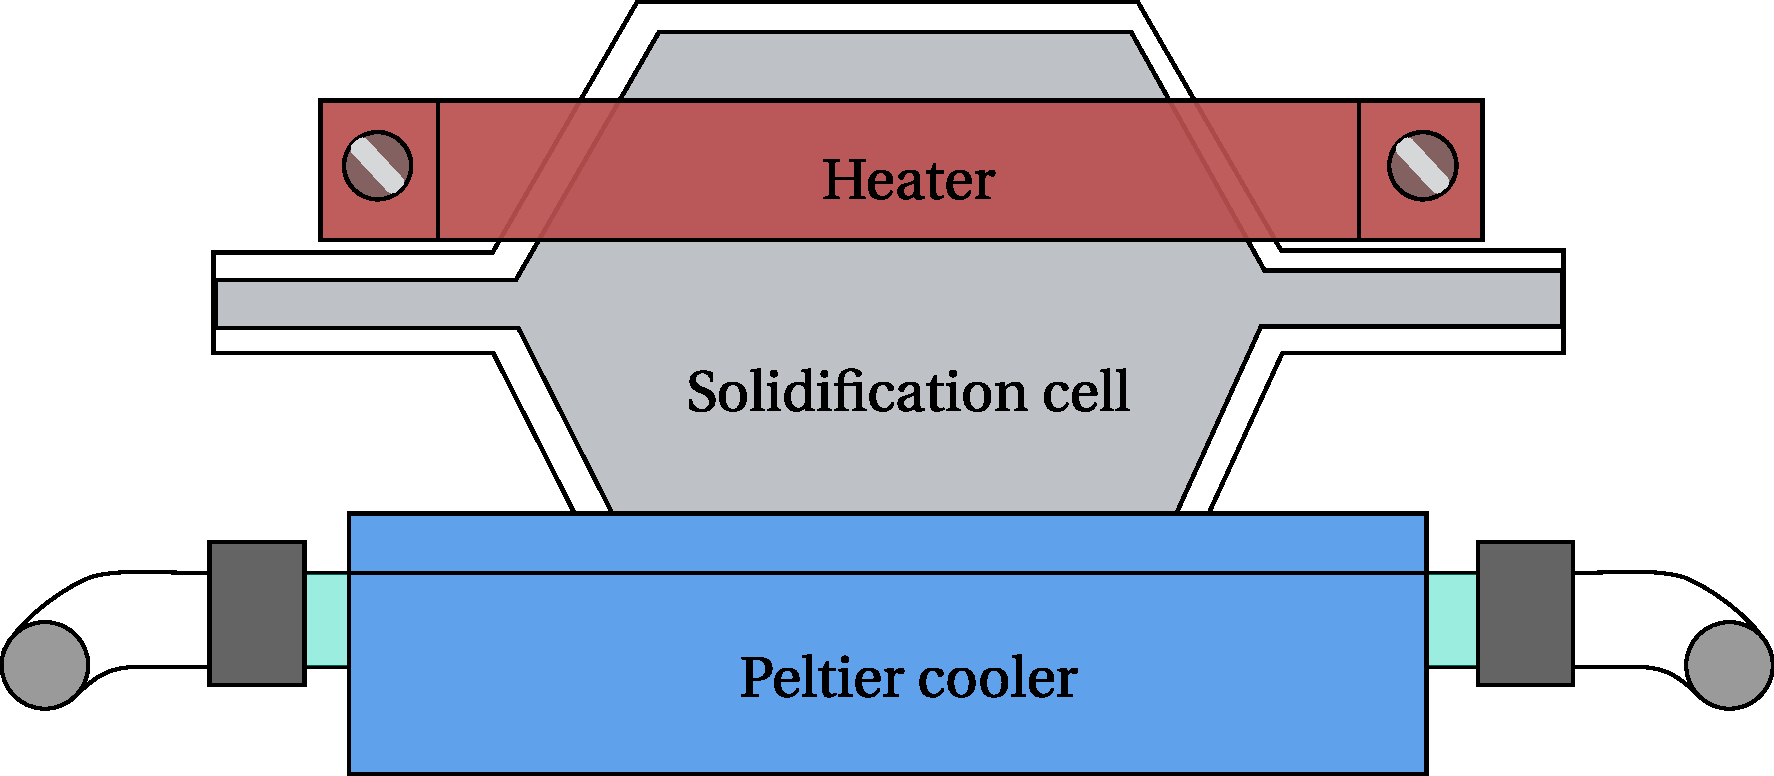
\includegraphics[height=3.5cm]{Chapter3/Graphics/freckle_exp/setup.pdf}
	\caption{}
    \label{fig:experimental_setup}
  \end{subfigure}
   %------------------------------
  \vskip\baselineskip
  %------------------------------
  \begin{subfigure}{0.5\textwidth}
    \centering
	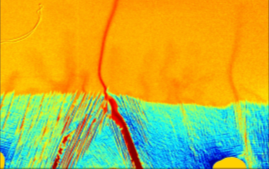
\includegraphics[height=4cm]{Chapter3/Graphics/freckle_exp/img.png}
	\caption{}
    \label{fig:experimental_img}
  \end{subfigure}
   %------------
\caption{Illustration of the benchmark experiments for in-situ observation of freckle 
formation using X-Ray radiography with (a) a schematic of the cell and (b) a typical image 
of the microstructure formed during directional solidification of an \bin{In}{75}{Ga} alloy. Reproduced from \citep{shevchenko_chimney_2013}.} 
\label{fig:experimental_freckles}
\end{figure}
%-----------------
%
%--------------------------
\subsection{Macroscopic scale simulations}
%
\subsubsection{Configuration}
%
%-----------------------
\begin{figureth}
{0.6}
{Chapter3/Graphics/freckle_fe/phasediagram/PhaseDiagram.pdf}
{Binary phase diagram of the In-Ga system \citep{andersson_thermo-calc_2002,tcbin_tcbin:_2006} and its approximation for solidification studies with an \bin{In}{75}{Ga} alloy. 
The dashed and dotted lines are linear liquidus and solidus approximations near the nominal composition.}
\label{fig:phasediagram_InGa}
\end{figureth}
%-----------------------
%
%----------------
\begin{tabulate}
%
% caption 
{Material parameters for \bin{In}{75}{Ga} and numerical parameters.}
% label
{table:data_case_InGa}
% line separation (e.g. 1.5mm)
{0.6mm}
% column justification-number (e.g. |c|ll|)
{llll}
% header titles (should use the & sign to switch columns)
{\textbf{Parameter} & \textbf{Symbol} & \textbf{Value} & \textbf{Unit}}
% cells content (should use the & and // to switch columns and rows)
{
Nominal composition 			& $\avg{\Cnominal}$		& 75 					& \si{\ucomposition} 	\\ 
Liquidus temperature			& $T_l$ 				& \num{25.25} 			& \si{\udegC} 			\\
Segregation coefficient			& $\k$					& \num{0.0165}			& \si{\ucomposition \per \ucomposition} \\
Liquidus slope					& $m_l$					& \num{-2.73}			& \si{\udegK \per \ucomposition} \\
\hline
Gibbs-Thomson coefficient			&$\Gamma_{\text{GT}}$	&\num{2e-7}			& \si{\udegC \per \metre} 		\\ 	
Heat capacity (liquid and solid)	&$C_p$ 					&\num{380.74}		& \si{\umasscapacity} 		\\ 	
Enthalpy of fusion					&$L$ 					&\num{8.02d-4}		& \si{\umassenergy} 	\\ 	
Diffusion coefficient of Ga in liquid In 		& $\Dl$ 	& \num{1.525d-9} 	& \si{\udiffusivity}  	\\ 
Dynamic viscosity  				& $\mul$ 					& \num{2e-3} 		& \si{\uviscosity}  	\\ 
Thermal expansion coefficient 	& \betaT 					& \num{0.0978e-3} 	& \si{\ubetaT}  		\\ 
Solutal expansion coefficient 	& $\betawl$ 				& \num{1.44e-3} 	& \si{\ubetawl}  		\\  
Thermal conductivity in the solid & $\ks$ 					& \num{40} 			& \si{\uconductivity}  	\\ 
Thermal conductivity in the liquid & $\kl$ 					& \num{28} 			& \si{\uconductivity}  	\\ 
Dendrite arm spacing 			& $\lambda$ 				& \num{60e-6} 		& \si{\metre}  			\\ 
Density 						& $\rhoref$ 				& \num{6725} 		& \si{\udensity}  		\\ 
Reference composition			&$\wlref$					& \num{75} 			& \si{\ucomposition}  	\\
Reference temperature 			&$\Tref$					& \num{25.25} 		& \si{\udegC}  			\\
\hline 
Initial temperature 	& $T_{\text{init}}$ & \num{1395}	& \si{\udegC}  \\ 
Ingot diameter 			&   	& \num{25e-3} 	& \si{\metre}  \\ 
Ingot length 			&   	& \num{75e-3} 	& \si{\metre}  \\ 
\hline 
CA cell size			&		& \num{30e-6}		& \si{\metre}  \\ 
FE mesh size 			&  		& \num{140e-6} 	& \si{\metre}  \\ 
Time step 				& $\dt$ & \num{0.1} 	& \si{\second}
}
%
\end{tabulate}
%-----------------
%
\subsubsection{Results}
The first case labeled FE-G1R1L0 is a reference case that features a low gradient (G1), low cooling rate (R1), 
and without any lateral cooling (L0), ensuring that isotherms retain a planar shape. These simulation parameters 
defined in \textbf{Table 2}, result in a negligible fluid flow reaching a maximum velocity of \SI{4d-8}{\milli\uvelocity} in the bulk. 
Accordingly, the solidification front remains stable and follows the planar isotherms; no freckles are observed. 
The average composition field is thus only little modified in the mushy zone as shown in \textbf{Figure 3 }(mind the values of the scale limits). 
It is concluded that velocity in the bulk is not high enough to initiate instabilities. In the next case, FE-G1R1L1, 
a cooling flux with a constant and very low value of the heat transfer coefficient is imposed on both vertical lateral 
surfaces to initiate a downward fluid flow by thermal buoyancy. Once solidification starts, solute-rich regions start 
to appear on the sides of the domain. Despite the visible concentration difference between these lateral regions and 
the central mush seen in \textbf{Figure 3}, their diffuse and uniform aspect indicates no resemblance to freckles. We keep the 
same configuration but increase the vertical gradient from \SI{0.2}{\ugradT} (G1) to \SI{1.5}{\ugradT} (G2) in the case FE-G2R1L1. 
The isotherms become closer to each over hence reducing the depth of the mushy zone for the same time increment compared 
to the preceding case. The rejected gallium solute locally accumulates at several different positions in the mushy zone, 
stemming from the base of the cell, with a maximum of \SI{0.7}{\ucomposition}Ga above nominal composition. 
This is the consequence of segregation of gallium rich liquid being lighter than the above liquid bulk and creating an 
upward buoyancy force. The positive segregation and subsequent Ga-rich chimneys then rise up with an upward velocity 
component slightly greater than \SI{1}{\milli\uvelocity}.
%
%-----------------
\begin{figure}[htbp]
\centering
  %------------
  \begin{subfigure}{0.5\textwidth}
    \centering
	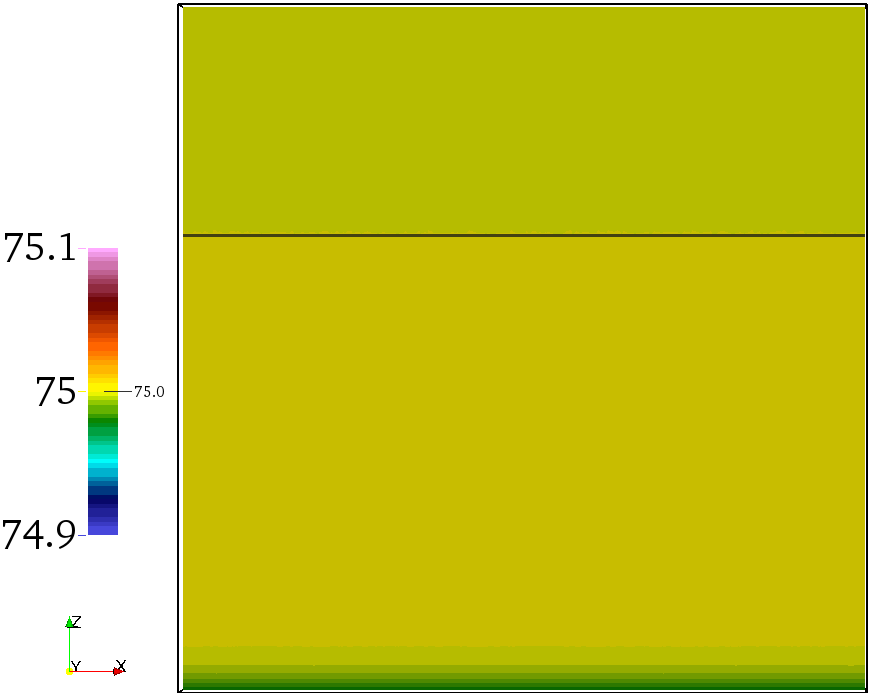
\includegraphics[width=\textwidth]{Chapter3/Graphics/freckle_fe/refA.png}
	\caption{FE-G1R1L0}
    \label{fig:refA}
  \end{subfigure}
   %------------------------------
  \vskip\baselineskip
  %------------------------------
  \begin{subfigure}{0.5\textwidth}
    \centering
	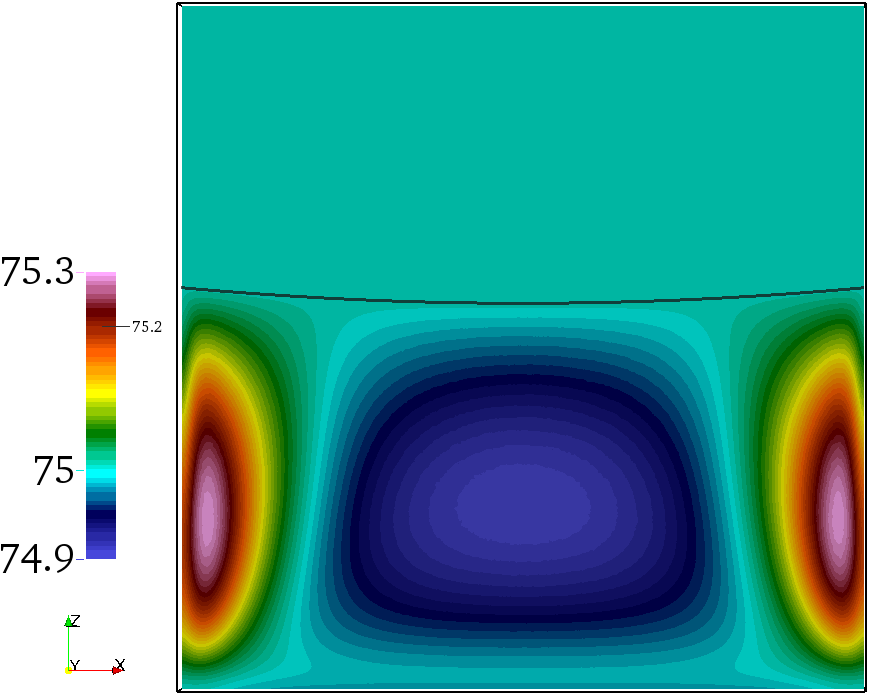
\includegraphics[width=\textwidth]{Chapter3/Graphics/freckle_fe/refB.png}
	\caption{FE-G1R1L1}
    \label{fig:refB}
  \end{subfigure}
   %-----------
  \vskip\baselineskip
  %------------------------------
  \begin{subfigure}{0.5\textwidth}
    \centering
	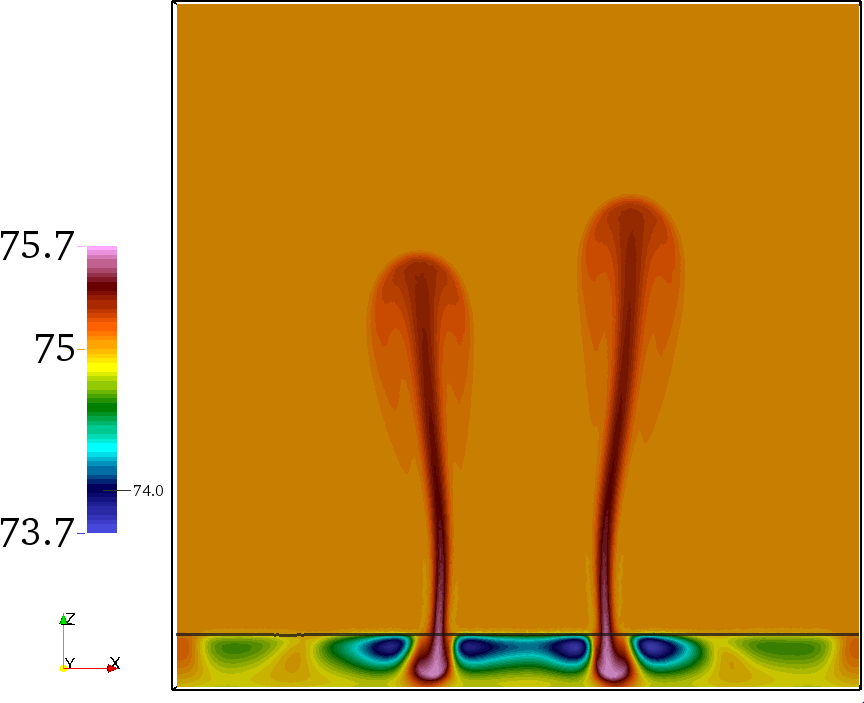
\includegraphics[width=\textwidth]{Chapter3/Graphics/freckle_fe/refC.png}
	\caption{FE-G2R1L1}
    \label{fig:refC}
  \end{subfigure}
   %------------
\caption{Average Ga composition field at \SI{250}{\utime} for the 3 FE cases showing the influence of 
process parameters on the freckling tendency. The black line represents the liquidus isotherm given in \cref{table:data_case_InGa}.} 
\label{fig:freckles_fe}
\end{figure}
%-----------------
%
\textbf{Figure 4} gives a series of snapshots for case FE-G2R1L1 at three different times. Among the two clear distinct 
plumes that are visible at \SI{250}{\utime} in \textbf{Figure 3}, only one has led to the formation of a freckle that remains in \textbf{Figure 4} at 
\SI{500}{\utime}. In fact, an animation between \SI{250}{\utime} and \SI{500}{\utime} (not shown here) reveals that one plume vanishes, 
thus permitting the first one to further develop. A second freckle is also seen on the left hand side of the cell. 
These two freckles are stable for a long time since they remain at time \SI{1000}{\utime}. However, the left side freckle 
develops further to become the main one at \SI{1500}{\utime}, while the mid-width freckle decreases in intensity, changes 
orientation and subsequently disappears (not shown here). Thus, the birth and death of very few freckles is observed in this 
simulation, mainly due to solutal instability, as the temperature field shown in \textbf{Figure 4 }clearly remains stable despite 
the low lateral heat flux. As shown in \textbf{Figure 3}, instability is yet required to create these chemical plumes and channels. 
Here, it is created by a very small lateral heat flow but other sources of instability could be involved, as shown with the grain structure in the next section.

\subsubsection{Discussion}
In the literature, many successful attempts have been made to predict freckles since (for example CITE fellicelli, poireau) ... 
until coming to kohler thesis results in 2008. These authors tackled the problem from an qualitative perspective. 
To our knowledge, the only close-to-quantitative work in solidification literature was done by \citet{ramirez_evaluation_2003}, 
who attempted to draw a correlation (freckling criterion) between the process parameters and the occurence of freckles, 
(without any size or shape constraints, i.e. any flow instability that may appear and form the smallest freckle is considered). 
To accomplish this, they took a number of experiments done independently by \citet{pollock_breakdown_1996} and \citet{auburtin_freckle_2000} 
where the casting parameters vary one at a time: casting speed (R), thermal gradient (G), angle ($\theta$) with respect to vertical 
orientation and nominal composition ($\avg{w_0}$), giving a database for 6 different superalloys. The experimental results were 
compared to a modified Rayleigh number that accounts for the various parameters. It allowed them to define a threshold for freckle 
formation in Nickel-base superalloys, as well as Pb-Sn alloys.
\comment{ They have also investigated Pb-Sn alloys, check }
Other contributions by \citet{yuan_new_2012} and  \citet{karagadde_3-d_2014} used a medium scale model to compare the simulated 
formation of freckles with the results obtained by \citet{shevchenko_chimney_2013} (explain at bit more)
However, all simulations show common traits in their predictions: (some words about the freckle dimensions, 
shape, intensity). These properties do not exactly meet with the experimental observations, just like in the 
In-Ga experiment. We think that the hydrodynamics scale at which freckles are born, is much smaller than the 
FEM scale. Since the relevant physics are not solved, even the finest FE mesh will not
be enough to see the exact grain boundaries. (now it is time to do transition to CAFE)
%
%-----------------------------------------------
\section{Meso-Macro freckle prediction}
%
\subsection{Configuration}
%----------------
\begin{tabulate}
%
% caption 
{Summary of the simulation cases with the corresponding parameters. 
The first series (FE-) consider the purely macroscopic model while the second series (CAFE-) 
makes use of the coupling with the grain structure model. Parameters are varied from (G1) low 
to (G2) high gradient, (R1) low to (R2) high cooling rate and (L0) no, (L1) low and (L2) high lateral cooling.}
% label
{table:data_simulation_InGa}
% line separation (e.g. 1.5mm)
{0.6mm}
% column justification-number (e.g. |c|ll|)
{cccccc}
% header titles (should use the & sign to switch columns)
%{\textbf{Case} & \textbf{Vertical gradient (G) \\ [\si{\ugradT}]} & \textbf{Cooling rate (R) \\ [\si{\uCR}]} & \textbf{Lateral cooling (L) \\ [\si{\uhconv}]}& \textbf{Nucleation \\ $(n_\text{max},\DeltaT_N,\DeltaT_\sigma)$ \\ [\si{\per\metre\square},\si{\udegK},\si{\udegK}]} & \textbf{Initial temperature} \\ (Top,Bottom) \\ [\si{\udegC}]
%}
{\textbf{Case} 
& \parbox{4cm}{\textbf{Vertical gradient}\\(G) \\ $K$} 
& sss 
& aaa 
& ffff & ffddfd}
% cells content (should use the & and // to switch columns and rows)
{
lll & ccc & sss & aaa & ffff & ffddfd \\ 
lll & ccc & sss & aaa & ffff & ffddfd}
%
\end{tabulate}
%-----------------
%
Knowing that the configuration in FE-G2R1L1 produces freckles, the same set of parameters is first used 
for case CAFE-G2R1L1 by adding the effect of the grain structure using the CAFE model. Results are accessible 
in \textbf{Figure 5} for comparison with \textbf{Figure 4}. A striking difference is seen: the composition maps become more 
perturbed as shown by the formation of numerous plumes when coupling with grain structure is active. The growing 
front displayed on the grain structure at the right most column of \textbf{ Figure 5} dictates the leading position of the 
mushy zone shown in the third column. Note that each color corresponds to one grain, with 17 grains having nucleated 
at the cell’s bottom surface. However, comparison of the solid fraction maps between \textbf{Figure 4} and \textbf{Figure 5} at the 
same times reveals a delay in the growing front position. Values of the nucleation parameters in \textbf{Table 3} are such 
that few grains rapidly form below the nominal liquidus isotherm. The delay is therefore not due to the nucleation 
undercooling but to the growth undercooling of the dendrite tips. It should be noticed that, the growth front driven 
by undercooling in \textbf{Figure 5} also forms with a higher initial solid fraction and hence larger solute segregation occurs 
at the front. This effect, together with instabilities of the composition field, is caused by a more perturbed fluid flow 
and more plumes as observed in CAFE-G2R1L1 compared to FE-G2R1L1. Such observations fit to the complicated fluid and solute 
flow patterns typically occurring in the experiments as shown in \textbf{Figure 6}. It becomes obvious that the consideration of grain 
structure and growth undercooling are vital to accurately simulate freckle formation in these experiments. The reasons for the 
instabilities are discussed hereinafter. In the present 3D CAFE simulation, each grain is associated with a crystallographic orientation. 
The growth kinetics is only given for the $\avg{100}$ crystallographic directions at the grain boundaries with the liquid. The CA growth model 
is based on the hypothesis that, in a quiescent liquid of uniform temperature distribution and composition, the grain envelop should 
reproduce an octahedral grain shape with main directions given by the six $\avg{100}$ directions. In the present situation where complicated 
fields are present for temperature, composition and liquid velocity, each grain envelope with different crystallographic orientation 
adapts differently to its local environment. Thus, the local undercooling of the front varies everywhere. Such variations are within 
few degrees here, but this is sufficient to create irregularities on the growth front, as seen on the grain structure in \textbf{Figure 5}. 
Apart from that, these variations are linked to the position of the instabilities for the chemical and liquid velocity fields, thus 
demonstrating the full coupling between the CA and FE models.
%
%
\subsection{Effect of vertical temperature gradient}
The influence of diverse process parameters can now be considered in context of the grain structure. 
The effect of the vertical temperature gradient is shown by comparing the previous case CAFE-G2R1L1 
with case CAFE-G1R1L1. The temperature gradient is decreased about 7 times here, from G2=\SI{1.5}{\ugradT}
to G1=\SI{0.2}{\ugradT}. In fact, both cases share almost all traits with respect to flow patterns and velocity
magnitude in the bulk. Main differences are yet seen regarding the dynamics of the plumes shown in 
\textbf{Figure 7}. In the case of a low temperature gradient (G1), the solidification front cannot maintain a 
shape as smooth as for the case of a large temperature gradient (G2): the solute gradient in the 
liquid of the mushy zone (basically following the lever rule approximation for a given temperature) 
decreases, leading to a lower gradient of the solutal buoyancy force. In turn, more solute accumulates 
close to the front and locally reduces the growth velocity, thus creating larger “valleys” or steps 
with higher solute content. The irregular geometry of the front is also influenced by the dendrite tip 
growth kinetics model. The velocity of the isotherms is the ratio of the cooling rate, R, to the 
temperature gradient, G. Consequently, the isotherm velocity in case G1 is larger than in G2, since 
cooling rate, R1, is the same in both cases. Moreover, because the dendrite tip velocity is a monotonously 
increasing function with the undercooling \citep{gandin_boundary_2003}, the latter for CAFE-G1R1L1 is larger 
than for CAFE-G2R1L1. Height differences of the growth front are proportional to the variations of the 
undercooling by the temperature gradient. Therefore, this forms larger steps on the growth front for case 
G1 compared to G2. The freckle extends deeper in the mushy zone when the temperature gradient increases. 
This is confirmed by both the simulation results shown in \textbf{Figure 7} as well as the experimental observations. 
Another remarkable phenomenon is also observed in the low gradient case: a “pulsing” mechanism in CAFE-G1R1L1 
where a series of solute rich liquid pockets are observed one above the other. This corresponds to a repeated
and localized strong spatial variation of the liquid velocity field outside the mushy zone, regularly thrusting 
away small plumes. These pulses are roughly similar to each other in size and exit speed, creating thus a very 
regular pattern during some time. In case of a high temperature gradient (case CAFE-G2R1L1) this phenomenon is 
barely seen. In fact, the pattern shown in Figure 7 is more typical, with continuous plume rising from the mushy 
zone and reaching the top of the domain. However, such regular plume is the initial and final pattern seen for low 
gradient before the pulsing regime. Similar observations have been made in the experiments too. \textbf{Figure 8(a)} displays 
the phenomenon of the “pulsing” plumes, which could be explained by the following mechanisms. The permeability of the 
mushy zone and the narrow gap of the solidification cell obstruct the feeding of the plumes by solute. A critical solute 
concentration has to be accumulated at a specific location in order to trigger the formation of a rising plume. An interim 
drop of the solute concentration below such a threshold would interrupt the plume. Flow instabilities can be another reason 
for the peculiar shape of the plumes. \textbf{Figure 8(b)} shows a pronounced continuous plume. The same plume can be seen a few seconds 
later in \textbf{Figure 8(c)}. The plume structure becomes unstable; one can observe an indentation of streamlines followed by a mixing of 
rising solute-rich liquid with descending In-rich fluid. This mechanism also causes a non-continuous structure of the plumes.
%
\subsection{Effect of cooling rate}
The next parameter studied is the cooling rate, corresponding to case CAFE-G1R2L1. A snapshot of the composition map 
and the corresponding vertical component of the velocity field are given in \textbf{Figure 9}. We see a similarity 
with case CAFE-G1R1L1 in \textbf{Figure 7} with respect to the buckled interface between the liquid and the mushy 
zone as well a plume pulsing effect when a low temperature gradient is applied. On the other hand, segregation inside 
the mush is more irregular with more pronounced patterns reaching a larger depth. One could distinguish alternating V  
and A shapes patterns in the mushy zone. As for case CAFE-G1R1L1, these patterns are created by a network of pulsing 
plumes formed by the steps created on the delocalized growth front due to the low temperature gradient. However, these 
considerations are not sufficient to explain the shape of the growth front. The reason for the protuberances created at 
the tips of the V shape is the presence of a descending bulk liquid with a low composition seen by the growth front. It 
infers that favorable growth conditions are created for a higher working temperature since the dendrite tip undercooling 
decreases for facing liquid flow and a lower composition; the growth rate is given by the isotherm velocity. The growth 
front thus adjusts its position to catch up with the corresponding isotherm, the latter being located at the tips of the 
V shape, i.e. the outmost advanced position of the growth front. It also means that the V shape angle depends on the size 
and intensity of the convection loops above the front. When the steps are formed on the growth front, the plumes exiting 
the mushy zone follow a direction normal to the front. They are inclined towards each other above the V shape. As a result, 
they may join and form a larger plume as seen in \textbf{Figure 7} CAFE-G1R1L1, thus forming larger and more stable freckles. 
The other observation in \textbf{Figure 9} is the existence of stable regions of the growth front. For instance, this is seen 
in between the two V shape forming or on the right hand side of the cell. The reason for this stability is the inversion of 
the composition gradient located ahead. Animation shows that solute coming from the top of the cell is responsible for this 
accumulation, creating a layering that provides a stabilization effect above the mushy zone. This is verified by the vertical 
component of the average velocity also made available in \textbf{Figure 9}. It is negative outside the path of the plumes. A resulting 
concurrent effect is the formation of the A shape segregates in between the V shape patterns seen in Figure 9. Finally, it can 
be observed that these patterns are sustained longer compared to \textbf{Figure 7} CAFE-G1R1L1 because, at high cooling rate, 
the flow in the mushy zone is decreased due to a faster solidification. This is the same effect as described for the large gradient 
configuration in \textbf{Figure 7} CAFE-G2R1L1.
It is not clear how these observations could be compared with the A  and V  shapes segregates reported for steel ingots 
\citep{pickering_macrosegregation_2013}. Despite the fact that macrosegregation is the main phenomenon leading to these 
patterns, there has not been a clear explanation yet in the literature for their formation. However, for steel casting, 
the A and V patterns are believed to form concomitantly. Further investigations would thus be required to quantify the 
consequences of thermosolutal instabilities simulated here for an \bin{In}{75}{Ga} alloy and check their possible correlation 
with experimental observations in steel casting.
%
\subsection{Effect of lateral temperature gradient}
The previous simulations show the effect of cooling rate and temperature gradient on the survival of segregation patterns deep 
in the mushy zone. Another simulation is performed by increasing the cooling rate using higher heat flux extracted from the 
vertical side boundaries. This is achieved in case CAFE-G1R1L2 where the heat transfer coefficient reaches \SI{500}{\uhconvec}. 
As a consequence of the large cooling from the sides, the temperature gradient is no longer vertical. A distinct flow due to 
thermal buoyancy is created, driving a cold liquid downwards near the sides of the cell. Under the influence of these 2 main 
convection loops, all segregation plumes tend to regroup in the middle of the domain, forming a larger central plume, as seen in 
the composition map at 450 s in \textbf{Figure} 10. However, this regime occurs at times earlier than 500 s, where the effect of thermally 
induced buoyancy forces is prevailing, feeding the convection loops. Approximately 500 s later, the mushy zone has extended, favoring 
the segregation mechanical forces i.e.  $\rhoref \brac{1-\betawl \Delta \wl} \gravity$, rather than the thermal mechanical forces, $\rhoref \brac{1-\betaT \Delta T} \gravity$. 
\textbf{Figure 10} shows the corresponding composition maps with stable freckles at about 1000 s that also remain at 1500 s. The solidification 
front then tends to form a concave shape at the center of the cell, thus partially revealing the form of the isotherms toward the cell 
center. The stable pattern in the center is similar to the plateau seen at the center of the A shapes in \textbf{Figure} 7 and \textbf{Figure} 9. As stated 
before, it is an inactive region with respect to plume initiation due to the inversion of the solute composition gradient. The composition 
field indeed shows accumulation of solute on top of the plateau in an established cuvette where no flow comes to destabilize the layering 
of solute. Outside of the plateau, 2 plumes are observed from the prominent instabilities of the growth front, adopting diverging directions. 
This is also observed at the center of the cell in \textbf{Figure} 9 on each side of the A shape segregate. These plumes in \textbf{Figure} 10 lead to the 
formation of two stable freckles. Liquid channels then form below the growth front.
The corresponding situation in the experiment is shown in \textbf{Figure} 11. The two freckles on both side and the plateau in between are clearly 
recognizable. The additional cooling at the side walls produces two flow vortices between the side wall and the strong plumes above the 
freckles. The central part of the sample remains almost unaffected by the additionally driven thermal convection. This area is characterized by 
the occurrence of a number of smaller plumes.  




